\chapter{Grafika}
\thispagestyle{chapterBeginStyle}
\label{chapter_graphics}

Ten rozdział traktuje o wy\'swietlaniu obiektów na ekranie i tworzeniu efektów specjalnych oraz cząsteczkowych.

Do wy\'swietlania grafiki w grze został użyty WebGL, rozwinięcie języka JavaScript, pozwalające wy\'wietlać obraz trójwymiarowy w przeglądarce. WebGL polega na używaniu shaderów, czyli programów wykonywanych na kartach graficznych. Język ten bazuje na języku OpenGL w wersji 2.0. WebGL jest tworzony przez Khronos Group, w skład którego wchodzą Mozilla, Apple, Google i Opera Software. W skład shaderów WebGL wchodzą dwa typy shaderów, vertex shader oraz fragment shader. Składnia jest podobna do języka C.\\
Typy danych dostępne w shaderach to:\begin{itemize}[topsep=0.2em, itemsep=0.5em, partopsep=0em, parsep=0em]
	\item bool, int i float, zachowujące się jak w zwykłym języku programowania
	\item [bi]vec2/vec3/vec4 - wektory wielko\'sci 2, 3 oraz 4 dla poprzednich typów - odpowiednio b to bool, i to int a brak przedrostka to float
	\item mat2/mat3/mat4 - macierze kwadratowe 2x2, 3x3, 4x4 ze zmiennymi typu float
	\item sampler2D - zmienna umożliwiająca dostęp do tekstury 2D
	\item samplerCube - zmienna umożliwająca dostęp do tekstury kostki
\end{itemize}
Można także używać struktur oraz tablicy zmiennych, jednak struktury nie mogą być używane z modyfikatorem varying. W shaderach można także używać wielu funkcji matematycznych i geometrycznych, są tu także dostępne proste operacje na macierzach i wektorach jak mnożenie lub dodawanie.

Dostępne modyfikatory to:\begin{itemize}[topsep=0.2em, itemsep=0.5em, partopsep=0em, parsep=0em]
	\item const - podobnie jak w języku C, jest to stała, tylko do odczytu
	\item attribute - dostepne tylko w vertex shaderze - oznacza zmienną w której można umie\'scić dane przekazane do shadera (po podzieleniu)
	\item uniform - podobnie jak modyfikator attribute, ten modyfikator pozwala umie\'scić w zmiennej dane z zewnątrz, jednak tutaj są one wspólne dla wszystkich przetwarzanych wierzchołków, nie są dzielone
	\item varying - dane otrzymane z vertex shadera, które zostaną w przetworzone w rasteryzatorze i podane dalej do fragment shadera (można w nich umie\'scić np. pozycje wierzchołków na teksturze, a zostanie otrzymana pozycja dla każdego z pikseli w otrzymanym kształcie)
\end{itemize}

Zazwyczaj jako zmienne z modyfikatorem uniform przekazywane są macierze przekształceń oraz \'swiatła, z modyfikatorem attribute przekazywane są dane do shadera, a modyfikatora varying używa się dla danych przekazywanych z vertex shadera do pixel shadera, na przykład pozycja tekstury. 
Specyfikacja języka WebGL jest opisana na stronie Khronos Group\cite{WebGLSpecification}. Bardzo przydatny podczas pisania programów jest też krótki dokument opisujący w skrócie język WebGL\cite{WebGLReferenceCard}.\newpage

\noindent{\LARGE Vertex shader}\smallskip

Vertex shader zajmuje się przetwarzaniem wierzchołków. Dane są przekazywane w całości, i dzielone na poszczególne wierzchołki automatycznie. Na przykład, je\'sli do wektora składającego się z 4 pól podamy ciąg długości 12, to zostanie on podzielony na dane dla 3 wierzchołków.
Następnie procesor wydaje polecenia mówiące o tym które wierzchołki mają zostać przetworzone i jaki kształt ma zostać użyty. O tym które wierzchołki będą przetworzone decydujemy, wybierając pierwszy wierzchołek i ich ilo\'sć.
Dostępne kształty to:\begin{itemize}[topsep=0.2em, itemsep=0.5em, partopsep=0em, parsep=0em]
	\item punkty (każdy wierzchołek utworzy jeden punkt o zadanej wielko\'sci)
	\item linie, w tym:\begin{itemize}[topsep=0.2em, itemsep=0.5em, partopsep=0em, parsep=0em]
		\item pomiędzy parami wierzchołków (każda para tworzy osobną linię)
		\item łamana otwarta (linia jest utworzona między danym wierzchołkiem i następnym dla każdego z wybranych wierzchołków)
		\item łamana zamknięta (tak jak poprzednio, ale łączone są też pierwszy i ostatni wierzchołek)
	\end{itemize}
	\item trójkąty, w tym:\begin{itemize}[topsep=0.2em, itemsep=0.5em, partopsep=0em, parsep=0em]
		\item każda trójka wierzchołków osobno
		\item wachlarz (dla każdego wierzchołka poza pierwszym bierze się dany wierzchołek, następny wierzchołek oraz pierwszy wierzchołek)
		\item pas (brane są dany wierzchołek oraz dwa następne)
	\end{itemize}
\end{itemize}
Przykładowo można narysować dwa trójkąty podając dane dla 6 wierzchołków, ale jeśli te trójkąty mają wspólny bok to mozemy zmniejszyć ilość wierzchołków podając jedynie 4 rogi i rysując je jako wachlarz. Można w ten sposób zmniejszyć ilość danych wysyłanych do karty graficznej co przyspiesza program.

W pixel shaderze istnieje specjalna zmienna gl\_Position, do której należy zapisać pozycję wierzchołka po przetworzeniu, a także zmienna gl\_PointSize, służąca do ustawienia wielko\'sci punktu, je\'sli rysujemy punkty.\bigskip

\noindent{\LARGE Fragment shader}\smallskip

Fragment shader zajmuje się przetwarzaniem pojedynczych pikseli. Dane w tym shaderze otrzymuje się z rasteryzatora i są one osobne dla każdego piksela, który zostanie narysowany na ekranie. Po obliczeniu koloru danego fragmentu (lub odrzuceniu go), kolor zapisuje się w zmiennej gl\_FragColor. W tym shaderze dostępna są także zmienne gl\_FragCoord typu vec4, pozycja fragmentu na ekranie, oraz gl\_FrontFacing typu boolean, mówiąca czy powierzchnia danego fragmentu jest zwrócona w stronę kamery.

We fragment shaderze zazwyczaj na podstawie pozycji z tekstury i innych danych, takich jak pozycja, kolor i typ \'swiatła, oblicza się kolor danego piksela.\bigskip

\noindent Przykładowy kod prostego programu shader:\smallskip

{\large Pixel shader}
\begin{lstlisting}
attribute vec2 position;
attribute vec3 color;

varying vec3 c;

void main(void) {
	c = color;
	gl_Position = vec4(position, 0.0, 1.0);
	gl_PointSize = 10.0;
}
\end{lstlisting}\newpage

{\large Fragment shader}
\begin{lstlisting}
precision mediump float;
#define defaultAlpha 1.0

varying vec3 c;

void main(void) {
	gl_FragColor = vec4(c, defaultAlpha);
}
\end{lstlisting}
\begin{figure}[h]
	\centering
	\noindent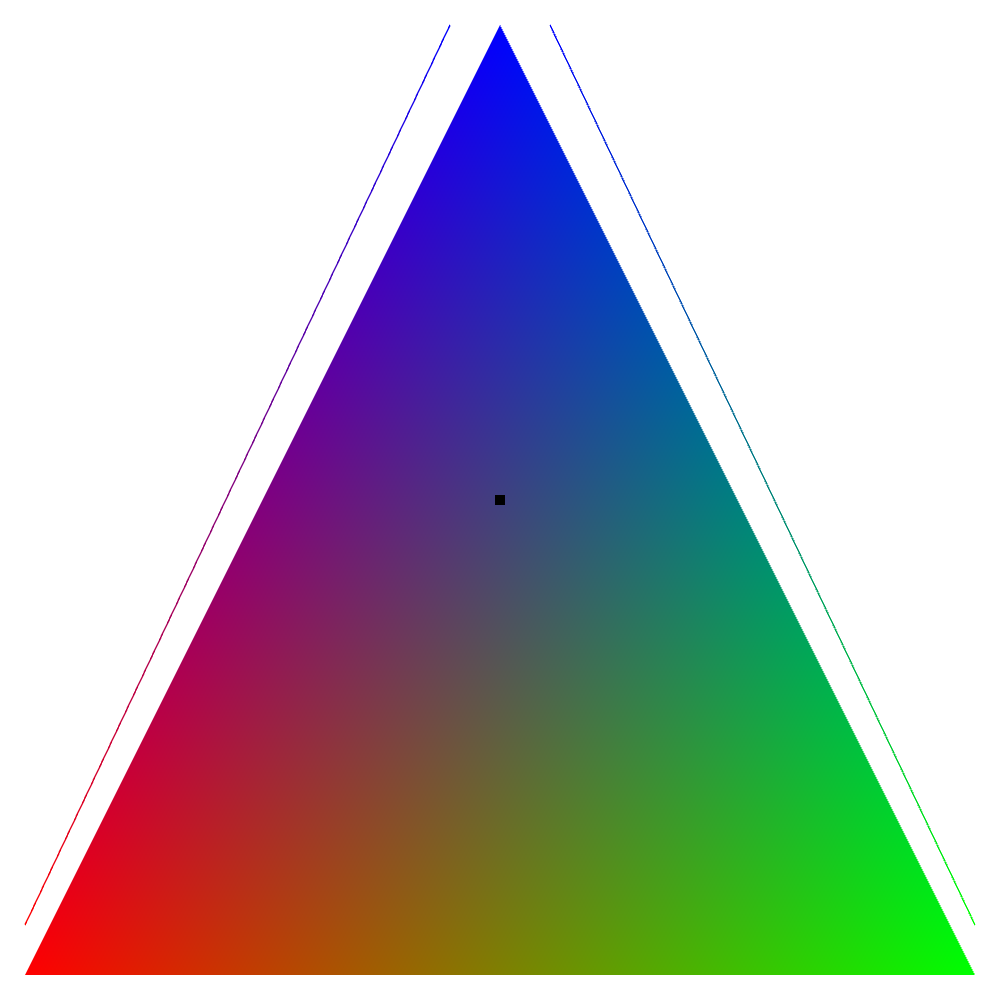
\includegraphics[width=\textwidth]{simple_shader}
	\caption{Wynik narysowania trójkąta, dwóch linii i punktu wielko\'sci 10 w przykładowym shaderze (szeroko\'sć punktu w oryginale to 10 pikseli)}
\end{figure}\vfill

\newpage\noindent{\LARGE Przykładowe shadery z efektami}

Zaprezentuję tutaj kilka shaderów tworzących ciekawe efekty. Można ich użyc jako efekty nałożone na całą scenę lub tylko no niektóre jej elementy, czasami też efekty same w sobie tworzą ładną grafikę.
Działają one w ten sposób, że kolor danego piksela jest obliczany jedynie na podstawie jego pozycji, używając funkcji matematycznych. Ze względu na działanie podzieliłem je na kształty oraz kolory.

\noindent{\Large Kształty}

Kształty dają jako wynik liczbę, przez którą mnożomy kolor dla danego piksela, aby wzmocnić lub osłabić w nim kolor.

\begin{wrapfigure}{r}{0.3\textwidth}
	\centering
	\noindent
\includegraphics[width=0.3\textwidth]{shape_rounded_square}
	\caption{Przykład zaokrąglonego kwadratu dla potęg 0.5, 1, 2 i 4}
	\noindent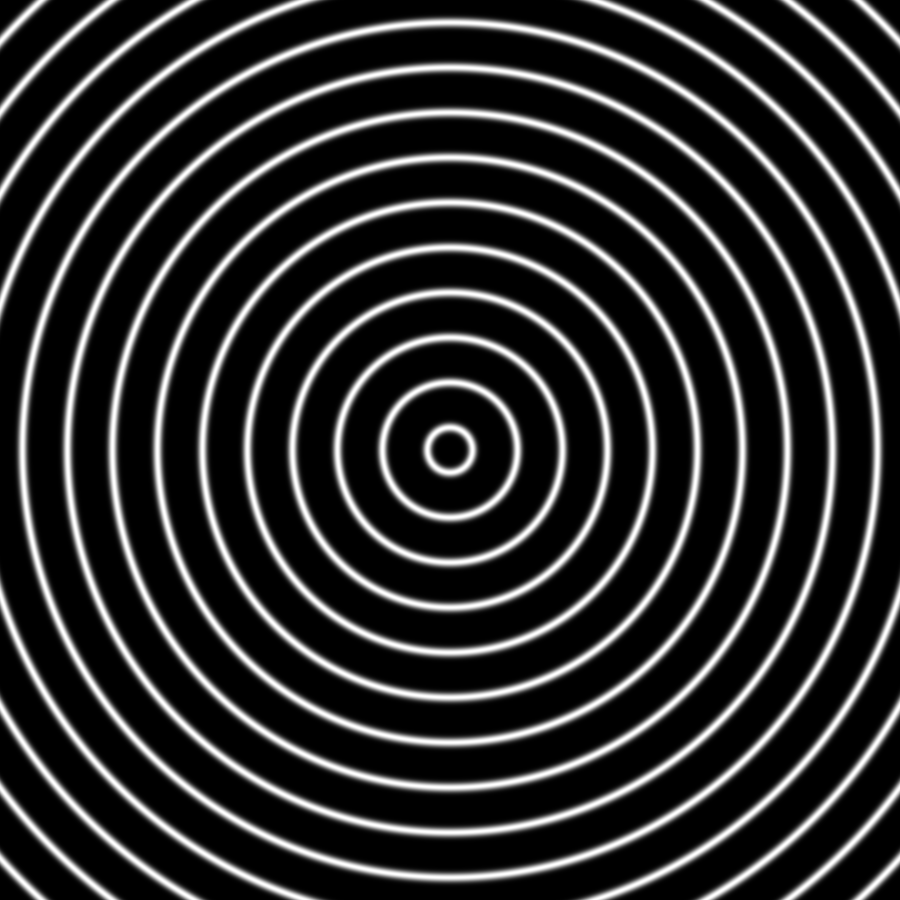
\includegraphics[width=0.3\textwidth]{shape_circles}
	\caption{Przykład efektu rozchodzących się kół}
\end{wrapfigure}
{\large Zaokrąglony kwadrat}

Uzyskuje się go przez obliczenie odległo\'sci za pomocą miary używającej innej potęgi (dla potęgi równej 2 uzyskuje się koło). Przy uzależnieniu stopnia potęgi od czasu można uzyskać ładny efekt pulsowania.

{\large Rozchodzące się koła}

Ten efekt uzyskuje się przez pomnożenie odległo\'sci od \'srodka przez jaką\'s stałą, dodanie aktualnego czasu, a następnie użycie na wyniku funkcji okresowej, takiej jak sinus. Aby uzyskać efekt perpektywy i tunelu można też użyć logarytmu z odległo\'sci.


\cleardoublepage